\subsection{Muon System}
Muons traverse the CMS detector with minimal interaction, and make up the majority of the visible particles that emerge through the calorimeter systems. This provides an opportunity to improve the identification, momentum resolution, and charge determination of muons by placing a final detector beyond the calorimeters. The CMS muon system is embedded in the return yoke of the solenoid magnet and covers the pseudorapidity $\abs{\eta}<2.4$. A schematic showing the layout of the muon system is given in \cref{fig:muon_system}.

\begin{figure}
  \centering
  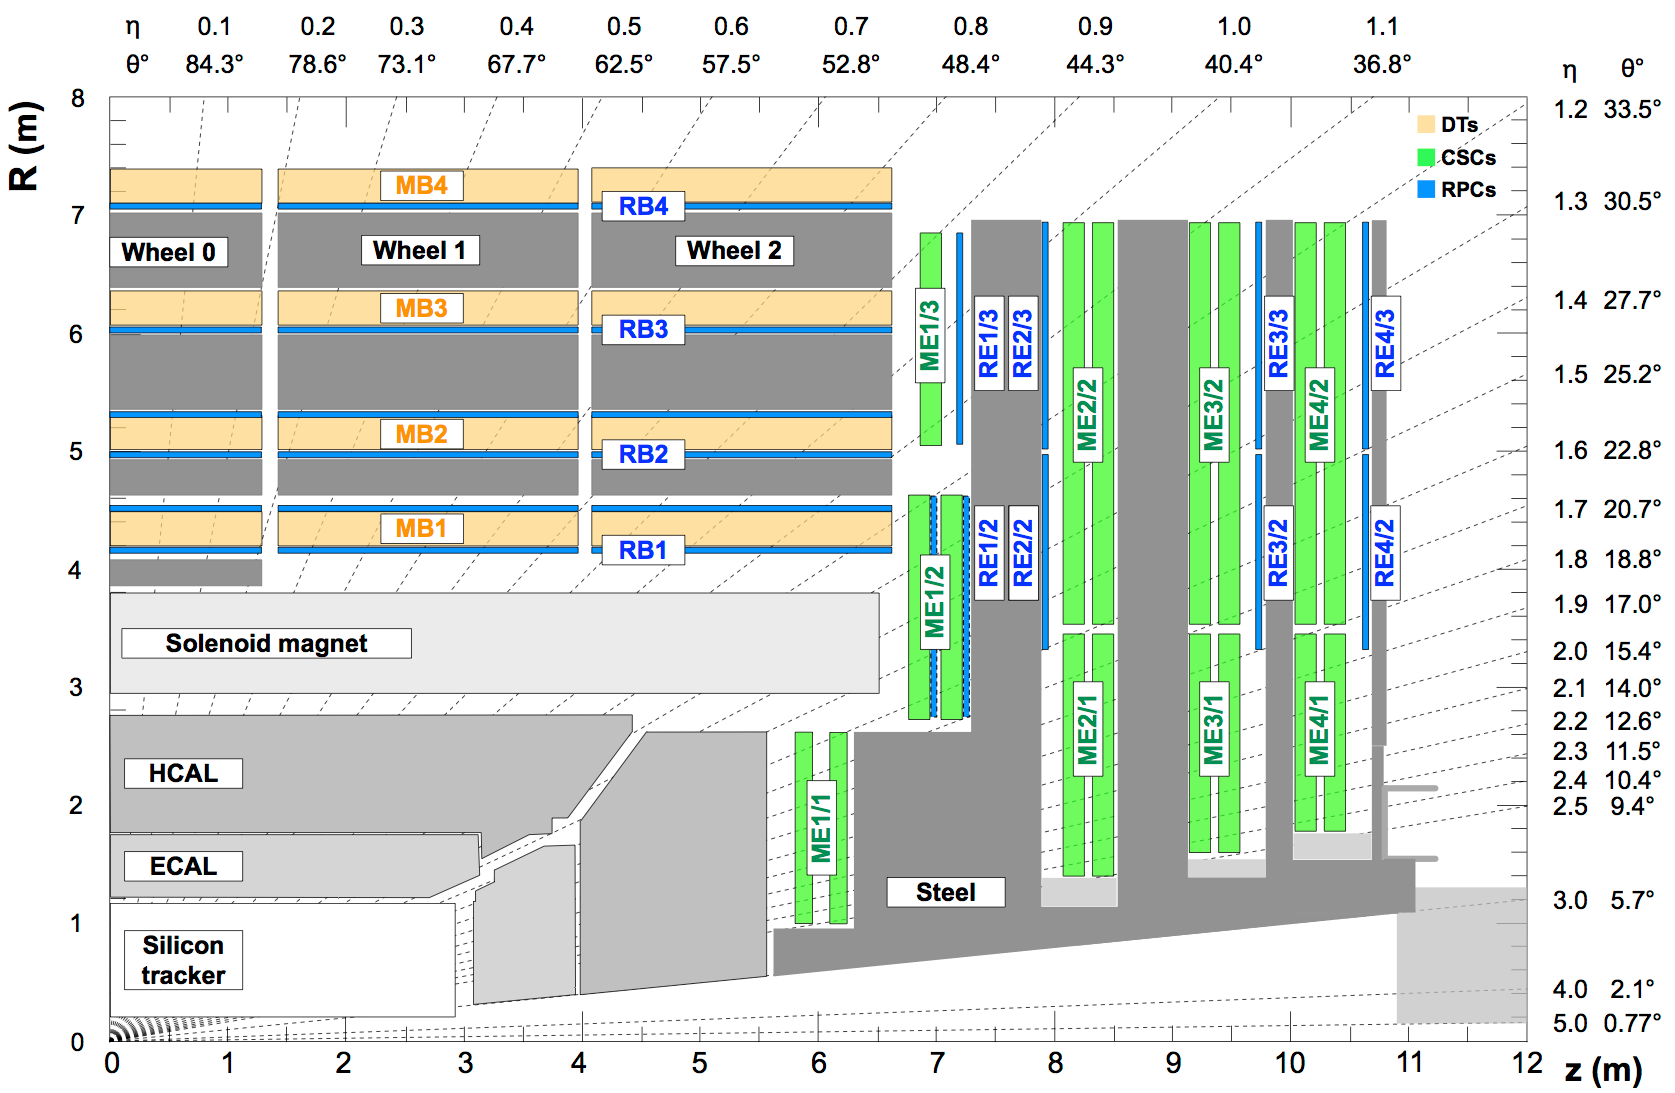
\includegraphics[width=\textwidth]{Figures/Detector/CMS/muon.pdf}
  \caption[The CMS Muon System]{A schematic of one quarter of the CMS muon system in the $r$-$z$ planes. The interaction point is the lower-left corner of the diagram and the dashed lines represent constant lines of $\eta$ and $\theta$. Figure taken from Ref.~\cite{CMS:2018rym}.}\label{fig:muon_system}
\end{figure}

The muon system is composed of layers of gaseous detectors which provide multiple measurements of a muon's trajectory. In the barrel, covering the $\abs{\eta}<1.2$ region, drift tube (DT) chambers are used. The chambers are made from $42 \times 13~\unit{mm^2}$ drift cells with wires arranged either parallel to the beam line or perpendicular depending on which layer the cells are in, thereby providing a measurement in the $r$-$\phi$ or $r$-$z$ plane respectively~\cite{CMS:2013vyz}.

In the endcap regions, cathode strip chambers (CSC) are installed and cover a range $0.9 < \abs{\eta} < 2.4$. The CSCs are multi-wire proportional chambers with cathode strips and anode wires arranged perpendicular to each other which provide measurements in the $r$-$\phi$ plane and of $\eta$ respectively. A third type of gaseous detector, resistive plate chambers (RPC), are used in both the barrel and endcaps in the $\abs{\eta} < 1.9$ range. These detectors have a fast response time and are primarily used to provide timing information to the muon trigger. 

Using this system, muons with $\pt > 30\GeV$ can be identified with an efficiency greater than 95\% with a misidentification rate of less than 1\%. Furthermore, for muons with $\pt < 200\GeV$, the momentum resolution is better than 3\%, and for muons with $200 > \pt > 1000\GeV$, where the addition of the muon system is especially beneficial, a resolution of 6\% or better is found~\cite{CMS:2018rym}.